%\documentclass{article}
%\usepackage[utf8]{inputenc}
%\title{test}
%\author{paolo.dini }
%\date{June 2017}
%\begin{document}
%\maketitle
%\section{Introduction}
%\end{document}

%===================================================
%================== DOCUMENT CLASS
%===================================================
\documentclass[runningheads,11pt,a4paper,english,llncs]{Misc/llncs}

%===================================================
%================== PACKAGES
%===================================================
%------------------------------------------------------------------------
% TeX and LaTeX macros
%------------------------------------------------------------------------
%
% In math formulas we use italic instead of mathitalic
%
\makeatletter
% ~ gives a \; space in math mode
\def~{\ifmmode\;\else\penalty\@M\ \fi}
%  Italic in mathematical formulas
\def\@setmcodes#1#2#3{{\count0=#1 \count1=#3
  \loop \global\mathcode\count0=\count1 \ifnum \count0<#2
  \advance\count0 by1 \advance\count1 by1 \repeat}}
\DeclareSymbolFont{italic}{OT1}{\rmdefault}{m}{it}
\let\mathit\undefined
\DeclareSymbolFontAlphabet{\mathit}{italic}
\edef\@tempa{\hexnumber@\symitalic}
\@setmcodes{`A}{`Z}{"7\@tempa41}
\@setmcodes{`a}{`z}{"7\@tempa61}
\makeatother
%
% \begin{asm} ... \end{asm}
%
\newdimen\asmindent     
\asmindent=\parindent
\newcount\asmi
\def\inc{\global\advance\asmi by 1}
\def\dec{\global\advance\asmi by-1}
\def\nl{{}$\par\hangindent\asmi em
  \noindent\kern\asmi em\ignorespaces$} 
\def\asmskip{{}$\par\smallskip\hangindent\asmi em
  \noindent\kern\asmi em\ignorespaces$} 
\def\asm{\global\asmi=0 
%%%%%%%%%%%%%% added by Paolo:
\parskip=0pt
%%%%%%%%%%%%%%%%%%%%%%%
 \def\+{\inc\nl}
 \def\-{\dec\nl}
 \def\\{\nl}
 \begin{trivlist}\item[]\leftskip=\asmindent\relax$}
\def\endasm{$\end{trivlist}}
%\mathindent=\asmindent
%
% \begin{asmarray}
%    f(s_1) & := t_1 \\
%    f(s_2) & := t_2 
% \end{asmarray}
%
\def\asmarray{\begin{array}[t]{@{}l@{\;}l@{\;}l@{}}}
\def\endasmarray{\end{array}}
%
%
%
\def\asmcomment#1{\quad\hbox{// #1}}
%
%  \begin{subasm} ... \end{subasm}
%
\newcount\asmii
\def\subasm{\vtop\bgroup\asmii=0\normalbaselines
 \def\nl##1{$\egroup\advance\asmii by##1\relax\hbox\bgroup\hskip\asmii em$}
 \def\\{\nl{0}}
 \def\+{\nl{1}}
 \def\-{\nl{-1}}
 \hbox\bgroup\hskip\asmii em$}
\def\endsubasm{$\egroup\egroup}
%
% Keywords in ASM code
%
\def\ASM#1{\hbox{\sc#1}}        % rule names and macros
\def\ASMIND#1{\ASM{#1}\index{#1@{\sc#1}}}
\def\AWAIT   {\mathrel{\mathbf{await}}}
\def\AND     {\mathrel{\mathbf{and}}}
\def\CASE    {\mathrel{\mathbf{case}}}
\def\CHOOSE  {\mathrel{\mathbf{choose}}}
\def\CREATE  {\mathrel{\mathbf{create}}}
\def\NEW  {\mathrel{\mathbf{new}}}
\def\DO      {\mathrel{\mathbf{do}}}
\def\ELSE    {\mathrel{\mathbf{else}}}
\def\ELSEIF  {\mathrel{\mathbf{elseif}}}
\def\FORALL  {\mathrel{\mathbf{forall}}}
\def\FORSOME  {\mathrel{\mathbf{forsome}}}
\def\FOREACH  {\mathrel{\mathbf{foreach}}}
\def\FROM  {\mathrel{\mathbf{from}}}
\def\THEREISNO  {\mathrel{\mathbf{thereisno}}}
\def\IF      {\mathrel{\mathbf{if}}}
\def\IFF      {\mathrel{\mathbf{iff}}}
\def\IMPORT  {\mathrel{\mathbf{import}}}
\def\IN      {\mathrel{\mathbf{in}}}
\def\LET     {\mathrel{\mathbf{let}}}
\def\SELF    {\mathrel{\mathbf{self}}}
\def\MATCH    {\mathrel{\textbf{match}}}
\def\NOT     {\mathrel{\mathbf{not}}}
\def\OF      {\mathrel{\mathbf{of}}}
\def\OR      {\mathrel{\mathbf{or}}}
\def\PAR     {\mathrel{\mathbf{par}}}
\def\SEQ     {\mathrel{\mathbf{seq}}}
\def\SKIP    {\mathrel{\mathbf{skip}}}
\def\THEN    {\mathrel{\mathbf{then}}}
\def\TO  {\mathrel{\mathbf{to}}}
\def\WHERE   {\mathrel{\mathbf{where}}}
\def\WHILE   {\mathrel{\mathbf{while}}}
\def\UNDEF   {\mathrel{\mathbf{undef}}}
\def\UNTIL   {\mathrel{\mathbf{until}}}
\def\WHEN   {\mathrel{\mathbf{when}}}
\def\WITH    {\mathrel{\mathbf{with}}}
\def\STEP    {\mathrel{\mathbf{step}}}
\def\STEPWISE    {\mathrel{\mathbf{stepwise}}}
\def\SEQ    {\mathrel{\mathbf{seq}}}
\def\RESULT  {\mathrel{\mathbf{result}}}
\def\CALL  {\mathrel{\mathbf{Call}}}
\def\LOCAL    {\mathrel{\mathbf{local}}}
\def\ADDGUARD {\mathrel{\mathbf{addGuard}}}
\def\ADDUPD   {\mathrel{\mathbf{addUpd}}}
\def\ADDRULE  {\mathrel{\mathbf{addRule}}}
\def\MINUSRULE  {\mathrel{\mathbf{minusRule}}}
\def\TO      {\mathrel{\mathbf{to}}}
%
% Including figures
%
\def\includefig#1#2{\centering\medskip
  \includegraphics[scale=#1]{fig/#2}
  \medskip}
%
% References to paragraphs in the ECMA standard for C#
%
\def\ecma#1{\cite[\S#1]{ecma334}}
%
%  Environments for definitions and theorems
%
%\theorembodyfont{\rm}
%\newtheorem{definition}[subsection]{Definition}
%\newtheorem{lemma}[subsection]{Lemma}
%\newtheorem{theorem}[subsection]{Theorem}
%\newtheorem{proposition}[subsection]{Proposition}
%\newtheorem{corollary}[subsection]{Corollary}
%\newtheorem{example}[subsection]{Example}
%\newtheorem{remark}[subsection]{Remark}
%\newtheorem{constraint}[subsection]{Constraint}
\def\proof{\trivlist\item[]{\bf Proof.}}
\def\endproof{$\Box$\endtrivlist}
%
% enumerate and itemize (smaller skips) from "latex.ltx"
%
\makeatletter
\def\enumerate{%
  \ifnum \@enumdepth >\thr@@\@toodeep\else
    \advance\@enumdepth\@ne
    \edef\@enumctr{enum\romannumeral\the\@enumdepth}%
      \expandafter
      \list
        \csname label\@enumctr\endcsname
        {\usecounter\@enumctr\def\makelabel##1{\hss\llap{##1}}
         \itemsep 0pt\parskip 0pt\parsep 0pt\topsep\smallskipamount}%
  \fi}
\def\itemize{%
  \ifnum \@itemdepth >\thr@@\@toodeep\else
    \advance\@itemdepth\@ne
    \edef\@itemitem{labelitem\romannumeral\the\@itemdepth}%
    \expandafter
    \list
      \csname\@itemitem\endcsname
      {\def\makelabel##1{\hss\llap{##1}}
       \itemsep 0pt\parskip 0pt\parsep 0pt\topsep\smallskipamount}%
  \fi}
\makeatother
%
% items in itemize
%
\def\bull{\vrule height .9ex width .8ex depth -.1ex}
\def\labelitemi{\bull}
%
%
%
\def\cs#1{C\#$_{\mathcal{#1}}$}
\def\lang#1{L$_{\mathcal{#1}}$}
%
% Positions
%
\def\pos#1{{}^{#1}}
\def\termPos{\blacktriangleright}
\def\cursor{\pos{\termPos}}
%
%
%
\def\sup{\hbox{sup}}
\def\c#1{\texttt{#1}}           % code
\def\N#1{\textit{#1}}           % non terminal symbols
\def\T#1{\hbox{`\texttt{#1}'}}  % terminal symbols
\def\A#1{\hbox{\sc#1}}          % ASM rules
\def\D#1{#1}                    % dynamic functions
\def\U#1{#1}                    % universes
\def\C#1{#1}                    % constructors
\def\rdef{\equiv}
\def\lbr{\c{\char`\{}}
\def\rbr{\c{\char`\}}}
\def\mb{\hbox{::}}
\def\map#1#2{\textbf{Map from}~#1~\textbf{to}~#2}
\def\cat{\cdot}
\def\adots{\mathinner{\ldotp\ldotp}}
%
%
% macros.tex ends here
\usepackage{etex}
\reserveinserts{28}
\newcommand{\todo}[1]{
 \noindent{\newline \color{red}
 \framebox[\textwidth][t]{%
  \parbox[t]{0.9\textwidth}{\textcolor{red}{TODO: #1}}                                                                                     
}}}


%===================================================
%================== PACKAGES
%===================================================
\usepackage{graphicx}
\usepackage{acronym}
\usepackage{ifthen}
\usepackage{substr}
\usepackage{color}
\usepackage{fixltx2e}
\usepackage[left=2cm, top=2cm, right=2cm, bottom=2cm]{geometry}
%\usepackage{subfigure}
\usepackage{array}  
\usepackage[figuresright]{rotating}          
\usepackage{url}
%\usepackage{enumerate}
\usepackage[shortlabels]{enumitem}
\usepackage{epsfig}
\usepackage{colordvi}
\usepackage{makeidx}
\usepackage{index}
\usepackage[absolute]{textpos}
\setlength{\TPHorizModule}{\paperwidth}
\setlength{\TPVertModule}{\TPHorizModule}
\textblockorigin{-6mm}{0mm}
\usepackage[%
      breaklinks=true,%
      colorlinks=true,%           no frame around URL
      urlcolor=LINK_COLOR,%            no colors
      menucolor=LINK_COLOR,%           no colors
      linkcolor=LINK_COLOR,%           no colors
      pagecolor=LINK_COLOR,%           no colors
      bookmarks=true,%            tree-like TOC
      bookmarksopen=false,%       expanded when starting
      hyperfootnotes=true,%       no referencing of footnotes, does not compile
      citecolor=CITE_COLOR,%           black cites
      filecolor=black,%           black files%
      hyperindex=true,%
      hyperfigures=true%
]{hyperref}
\usepackage{bookmark}
\usepackage{booktabs}
\usepackage{dsfont}
\usepackage{wallpaper}
\usepackage{mathtools,cancel}
\usepackage{soul}
\usepackage{float}
\usepackage{setspace}
%\usepackage{morefloats}
%\usepackage{mdwlist}
\usepackage{amsmath,amssymb,amscd,diagrams,bm,amsfonts}
\let\proof\relax
\let\endproof\relax
\usepackage{amsthm}
\usepackage{tabularx, graphics, longtable}
%TIKZ
\usepackage{tikz}
\usepackage{tikz-cd}
\usetikzlibrary{trees,snakes}
\usetikzlibrary{arrows,automata}
\usetikzlibrary{matrix,arrows,positioning}
\usetikzlibrary{mindmap,backgrounds}
\usetikzlibrary{shapes}
\usepackage{verbatim} %for comment out some texts


%%%%%%%%%%%%%%%%%%%%%%%%%%%%%%%
%%%%%%%%%%%%%%%%%%%%% Egon's commands:
\usepackage{latexsym}
\ifx\pdfoutput\undefined
  \message{We are running LaTeX.} 
%PD  \usepackage[dvips]{graphicx}
%PD  \DeclareGraphicsExtensions{.eps}
%PD  \usepackage[hypertex,bookmarks=false]{hyperref}
\else
  \message{We are running PDFLaTeX.}
%PD  \usepackage[pdftex]{color}
%PD  \usepackage[pdftex]{graphicx}
%PD\DeclareGraphicsExtensions{.jpg,.pdf}
%PD  \DeclareGraphicsExtensions{.pdf}
%PD  \usepackage[pdftex,bookmarks=false]{hyperref}
%PD  \hypersetup{colorlinks={true},
%PD            linkcolor={blue},
%PD            citecolor={blue},
%PD            urlcolor={blue},
%PD            plainpages={false}
%PD  }
\fi
%%%%%%%%%%%%%%%%%%%%%%%%%%%%%%%
%%%%%%%%%%%%%%%%%%%%%%%%%%%%%%%


%===================================================
%================== COLOURS
%==================================================

\definecolor{green}{rgb}{0,0.6,0} 
\definecolor{gray}{rgb}{0.6,0.6,0.6} 
\definecolor{red}{rgb}{1,0,0} 
\definecolor{blue}{rgb}{0,0,1} 
\definecolor{purple}{rgb}{0.5,0,0.5} 
\definecolor{yellow}{rgb}{0.25,0.25,0} 
\definecolor{turquoise}{rgb}{0,0.5,0.5}
\definecolor{brown}{rgb}{0.6,0.2,0.1}

\definecolor{LINK_COLOR}{rgb}{0,0,0.7}
\definecolor{CITE_COLOR}{rgb}{0,0.5,0}
\definecolor{lightblue}{rgb}{0,0,1}
\definecolor{light-gray}{gray}{0.95}
\def\red#1{\textcolor[rgb]{1.0,0.0,0.0}{#1}}
\def\green#1{\textcolor[rgb]{0.0,0.8,0.1}{#1}}
\def\blue#1{\textcolor[rgb]{0.0,0.0,1.0}{#1}}

%===================================================
%================== LAYOUT
%===================================================
\parindent=0cm
%\setlength{\parskip}{1.0\baselineskip plus 0.5ex minus 0.2ex}
\abovecaptionskip=0cm
\hyphenpenalty=5000
\tolerance=1000 
\floatsep=1in
\allowdisplaybreaks
\def \constzeroindent {0cm}
\def \constfirstindent {0.5cm}
\def \constsecondindent {1cm}
\newenvironment{mycustomindent}[1]
{\setlength{\parindent}{#1}}
{\setlength{\parindent}{\constzeroindent}}
\newcommand{
	\firstindent}[1]{
	\begin{mycustomindent}{\constfirstindent}
	\begin{tabular}{@{}p{12cm}@{}}
	#1 \\
	\end{tabular}
	\end{mycustomindent}
}
\newcommand{
	\secondindent}[1]{
	\begin{mycustomindent}{\constsecondindent}
	\begin{tabular}{@{}p{12cm}@{}}
	#1 \\
	\end{tabular}
	\end{mycustomindent}
}
\newenvironment{packed_item1}{
\begin{itemize}[topsep=0pt, partopsep=0pt]
  \setlength{\itemsep}{5pt}
  \setlength{\parskip}{0pt}
  \setlength{\parsep}{0pt}
}{\end{itemize}}
\newenvironment{packed_item2}{
\begin{itemize}[topsep=0pt, partopsep=0pt]
  \setlength{\itemsep}{0pt}
  \setlength{\parskip}{0pt}
  \setlength{\parsep}{0pt}
}{\end{itemize}}
\newenvironment{packed_enumerate}{
\begin{enumerate}[topsep=0pt, partopsep=0pt]
  \setlength{\itemsep}{5pt}
  \setlength{\parskip}{0pt}
  \setlength{\parsep}{0pt}
}{\end{enumerate}}
% The following commands are to get rid of the extra space around section and subsection titles:
% Save the class definition of \subparagraph:
\let\llncssubparagraph\subparagraph
% Provide a definition to \subparagraph to keep titlesec happy:
\let\subparagraph\paragraph
\usepackage[compact]{titlesec}
\usepackage{dblfloatfix,caption,subcaption}
\titlespacing{\section}{0pt}{12pt}{*0}
\titlespacing{\subsection}{0pt}{6pt}{0pt}
\titlespacing{\subsubsection}{0pt}{6pt}{0pt}
% Force section numbering to follow chapter numbering:
\usepackage{chngcntr}
\counterwithin{section}{chapter}
\counterwithin{figure}{chapter}
%\counterwithin{theorem}{chapter}
%\counterwithin{lemma}{chapter}
%\counterwithin{definition}{chapter}
%%%%%%%%%%%%%%%%%%%%%%%%%%%%
% Allow line breaks in long list of citations that would extend into the margin:
\usepackage{breakcites}
%%%%%%%%%%%%%%%%%%%%%%%%%%%%%%%%%%%%%%

\usepackage{pdfpages}
\pagestyle{headings}

\renewcommand{\rightmark}{INTERLACE Project (Grant no.~754494)}
\renewcommand{\leftmark}{D2.1}
\setcounter{tocdepth}{2}

\usepackage{tocloft}
\setlength\cftparskip{0pt}
\setlength\cftbeforechapskip{12pt}

\usepackage{abstract}
\renewcommand{\abstractnamefont}{\large \bfseries}
%\setlength{\abstitleskip}{-\absparindent}
\renewcommand{\abstractname}{Abstract}

\setlength{\parskip}{12pt}

\begin{document}
%===================================================
%================== TITLE
%===================================================

\thispagestyle{empty}
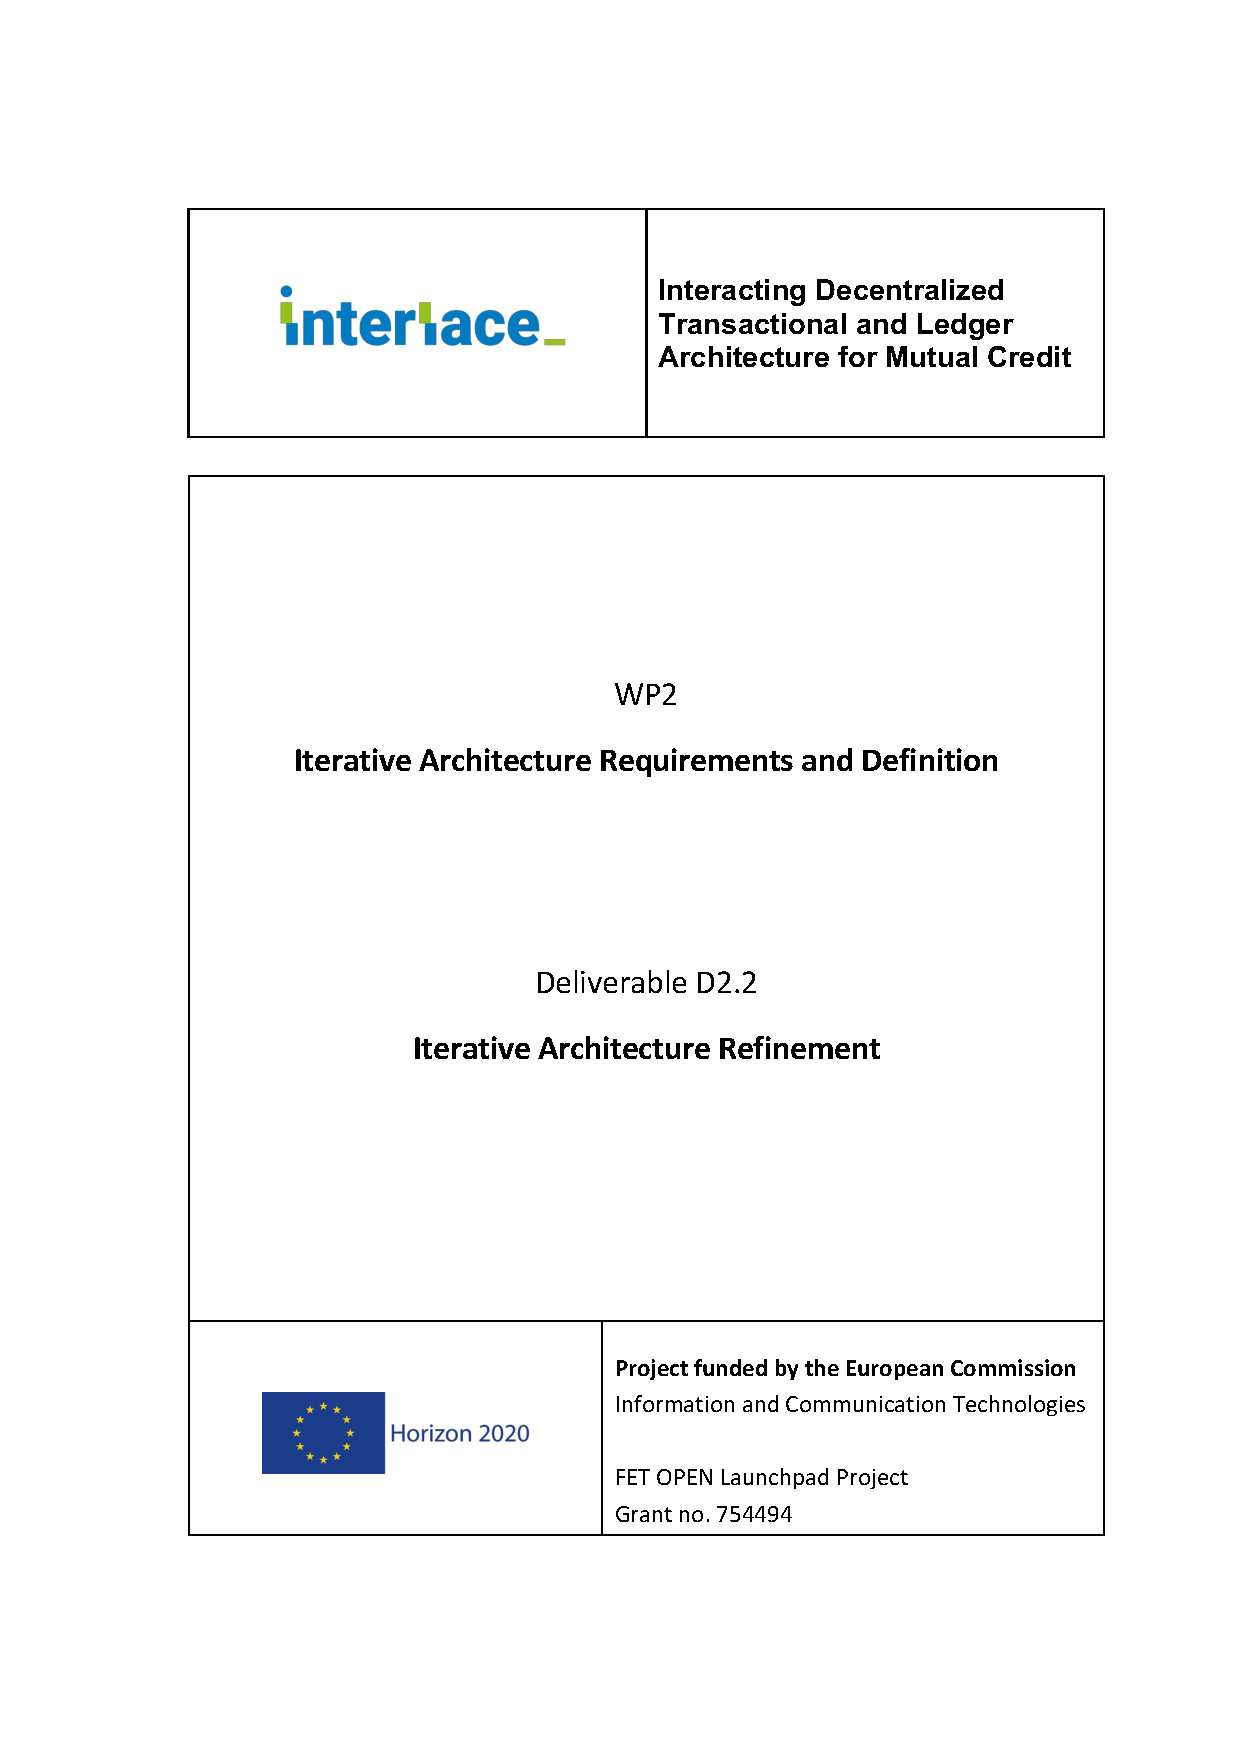
\includepdf[pages=-, scale=1.0]{Misc/Front}

%===================================================
%================== ABSTRACT
%===================================================
\thispagestyle{empty}

\begin{abstract}
\normalsize


\end{abstract}

\newpage

%===================================================
%================== TABLE OF CONTENTS
%===================================================
\tableofcontents

%===================================================
%================== CHAPTERS
%===================================================
\chapter{Introduction}
\label{ch:Introduction}

\vspace{-1cm}
\begin{center}
Paolo Dini and Giuseppe Littera
\end{center}

The selection of a blockchain technology for the INTERLACE platform has been a long and difficult process. The challenge has arisen from the wide variety of technologies, architectures, and protocols, from the very rapid rate of innovation in this field, and from the evolving requirements of a future vision for the Sardex platform. This is because, although INTERLACE is only a first attempt at a blockchain-based transactional platform for the Sardex circuit, it should be as compatible as possible with the future vision of the circuit.

The future vision of the Sardex circuit has been difficult to define because it took a long time to understand how the Sardex mutual credit system could scale to global level while remaining faithful to its principles of support for local economies and of reliance on trust between its users. Since the social and the business dimensions are the starting point for the requirements that lead to choice of technology and architecture definition, we adopted a circular and iterative approach that compared what was possible with what is desirable at each step, and slowly evolved the vision as our understanding of the blockchain space and of our own requirements improved. In this short report we cannot go into too much depth, but it is worth addressing what is arguably the central concept for both Sardex and the blockchain: trust.

\section{Sardex, Trust and the Blockchain}
The blockchain is often described as a `trustless' technology, since the distribution of the validation and record-keeping function to many independent nodes, together with cryptographic algorithms, removes the need for a central authority that plays the role of record keeper and transaction orderer. According to the prevailing view in Computer Science, therefore, trust in a central authority and bilateral trust between transacting parties are substituted for reliance on a type of technology and protocol. Clearly, such an approach is particularly useful in situations where there is not trust at all between transacting parties.

By contrast, the Sardex circuit relies on trust to a very significant extent. Between the ``sociological'' trust discussed by Sartori and Dini \cite{SartoriDini2016} and the trust in the technology platform lies an ``economic'' type of trust. In particular, Sardex relies on, and reinforces, ``thick trust''.\footnote{Richard Simmons, economist, private communication, 2018.} Thick trust has been discussed in the literature in the business context (e.g. \cite{VosselmanMeerKooistra2009}), but for our purposes it is sufficient to define it as the combination of ``Know Your Customer'' with ``Know Their Products''. The role of the Sardex company that runs the circuit, combined with the work of the Sardex brokers, greatly reduces the social cost of trust for the SMEs who participate in the network and achieves and combines both these components, because it is able to make trust transitive: the circuit members trust the Sardex company and the electronic platform, and in the majority of cases this trust extends to bilateral trust between the transacting parties, making the Sardex circuit a particularly strong and stable trading community.

One of the drawbacks of such an approach is that the communities and companies involved in the network ultimately depend on one actor to facilitate credit and trade among participants, rendering the network as a whole highly efficient yet vulnerable and not as inclusive and socially/financially adoptable as might be preferred.

Why, then, is Sardex interested in the blockchain? For two reasons. First, as the company operations grow beyond Sardinia and Italy to other countries in Europe and beyond they will involve interactions with other circuits whose legal personality, business relationship with Sardex, and proprietary structure may vary along a range of options depending on the context and stakeholders. Therefore, from a functional and organisational point of view it may be more expedient to build in some flexibility at the level of the architecture: for example, each circuit could run a separate node of the blockchain. This could enable inter-circuit trade via agreements recorded on distributed ledgers, more transparency of the overall network, and regional and local clusters of SMEs -- which in turn reduces informational asymmetries.

Second, this organisational flexibility requirement, which is essentially functionalist, is reinforced by the social and cultural requirement of respecting local community identity to the extent possible. This is not so much a matter of institutional or governance efficiency as a question of shared values built around reciprocal respect between different communities who identify with different regions or localities. We feel it is easier to meet such expectations with an articulated and decentralised\footnote{In contrast to what we wrote in the INTERLACE proposal, we have adopted the definition of `decentralised' as an architecture where control is distributed, as opposed to `distributed', which refers only to a distribution of functional aspects but leaves the control central.} architecture than through a monolithic platform like Facebook or Google.

\section{Overview of Report}
This brief report provides a high-level discussion of the main blockchain technologies we examined during the course of the project, together with a rationale for choosing Hyperledger as the core component with possible extensions towards Ethereum and Holochain. The discussion in the rest of the report assumes familiarity with the basic concepts and terminology of the main blockchain technologies as can be found, for example, in \cite{TascaEtAl2017}.

Chapter \ref{ch:dlt} discusses a few candidate Distributed Ledger Technologies (DLTs) that we assessed in the process of deciding which satisfied the INTERLACE and Sardex requirements best. The next step in the process was going to be an ASIM specification and CoreASIM modelling of the transactional platform, which would have been reported in a third chapter, but lack of funding complementary to INTERLACE made this plan impossible. We therefore decided that it made more sense to focus the remaining time and resources on implementing a proof-of-concept transactional platform based on the requirements specified in deliverable D2.1 \cite{INTERLACE_D21} and updated in deliverable D3.1 \cite{INTERLACE_D31}. The implementation work is reported in deliverable D3.2.



\section{Table of Acronyms}
Table \ref{acronyms} shows the definition of the acronyms used in this report.


\begin{table}
\begin{centering}
{\begin{tabular}{| r | c | l |}
\hline
AML		&& Anti Money Laundering\\
\hline
ASM		&& Abstract State Machine \\
\hline
ASIM	&& Abstract State Interaction Machine \\
\hline
B2B		&& Business-to-Business\\
\hline
B2C		&& Business-to-Consumer\\
\hline
BFT		&& Byzantine Fault Tolerance\\
\hline
BTC		&& Currency symbol for Bitcoin\\
\hline
Dapp	&& Distributed App\\
\hline
DB		&& Database\\
\hline
DHT		&& Distributed Hash Table\\
\hline
DLT		&& Distributed (or Decentralised) Ledger Technology\\
\hline
DoS		&& Denial of Service\\
\hline
ETH		&& Currency symbol for Ether, the Ethereum token\\
\hline
EVM		&& Ethereum Virtual Machine\\
\hline
FDAS	&& Federated Distributed Agreement System\\
\hline
FPML	&& Financial Products Markup Language\\
\hline
GDPR	&& General Data Protection Regulation\\
\hline
ICO		&& Initial Coin Offering\\
\hline
JS		&& Javascript\\
\hline
JVM		&& Java Virtual Machine\\
\hline
KYC		&& Know Your Customer\\
\hline
LE		&& Leader Election\\
\hline
PBFT	&& Plenum Byzantine Fault Tolerance\\
\hline
PoA		&& Proof of Authority\\
\hline
PoS		&& Proof of Stake \\
\hline
PoW		&& Proof of Work\\
\hline
QI		&& Quorum Intersection\\
\hline
REST 	&& Representational State Transfer\\
\hline
SC		&& Smart Contract\\
\hline
SCP		&& Stellar Consensus Protocol\\
\hline
SMR		&& State Machine Replication\\
\hline
SQL		&& Structured Query Language\\
\hline
SRD		&& Currency symbol for Sardex credits\\
\hline
Tx/s		&& Transactions per second\\
\hline
UML		&& Unified Modelling Language\\
\hline
UTXO	&& Unspent Transaction Output\\
\hline
XLM		&& Currency symbol for Lumen, the Stellar token\\
\hline
\end{tabular}}
\caption{\bf \small Table of acronyms used in the report}
\label{acronyms}
\end{centering}
\end{table}











\newpage












\chapter{Main Blockchain Technologies for INTERLACE}
\label{ch:DLTs}

\vspace{-1cm}
\begin{center}
Paolo Dini, ...
\end{center}

\section{Introduction}

bla bla


\section{Stellar}
\subsection{Introduction}
In this section we provide a mathematical summary of the Stellar Consensus Protocol (SCP) \cite{Mazieres2016}. The presentation involves a sequence of definitions interspersed with theorems and their proofs. Understanding the theorems and their proofs is essential to understanding the Stellar system and the SCP. Therefore, although we follow Mazi\`eres's paper \cite{Mazieres2016} very closely, we provide more elementary explanations of the mathematical formulation, relying on figures and diagrams created ad hoc as needed.

SCP is based on a new decentralized agreement system, also defined and developed in \cite{Mazieres2016}, called Federated Byzantine Agreement System (FBAS). FBAS and SCP, together, provide an alternative to Bitcoin's Proof of Work (PoW) \cite{Antonopoulos2015} or Ethereum's Proof of Stake (PoS) \textcolor{red}{[refs]} to achieve consensus. FBAS is a generalization of Byzantine agreement \textcolor{red}{[refs]} that is analogous to a permissioned system. Although the early implementation of the new Sardex INTERLACE platform will be permissioned, we wish to develop an architecture that can easily replace centralized control with local consistency between transacting parties. At the level above in the network hierarchy, we will also need to manage a federated network of circuits. Also here the capability to transition to a scalable decentralized architecture is preferable to a traditional centralized approach, although at this level Corda may be a more appropriate Distributed Ledger Technology (DLT) framework, as discussed in Section \ref{corda}.

\subsection{Federated Byzantine Agreement System}
A Stellar network relies on a FBAS to achieve consensus in the absence of central control. The consensus is on the update of replicated states such as ledger records corresponding to transactions. The purpose of the consensus protocol is for a set of nodes to reach agreement on a given update. Each update is identified with a unique \emph{slot} which also encodes information on inter-update dependencies -- for example as consecutively numbered positions in a transaction ledger. A FBAS runs a SCP that ensures that the nodes agree on slot contents. Agreement is defined in terms of safety of operation; the definition is somewhat recursive so it may need to be refined later:
\begin{defin}
We say that a node $v$ can \emph{\bf safely} apply update $x$ in slot $i$ when
\begin{packed_item1}
\item it has safely applied all the updates in all the slots upon which $i$ depends, and
\item it believes all correctly functioning nodes will eventually agree on $x$ for slot $i$.
\end{packed_item1}
\end{defin}
\smallskip
\begin{defin}
When node $v$ has safely applied update $x$ in slot $i$ we say that $v$ has \emph{\bf externalized} $x$ for slot $i$.
\end{defin}
The reason for this term is that once the contents of a slot have been accepted by other nodes they (the other nodes) could perform irreversible actions as a consequence, which $v$ cannot do anything about: the contents are now outside or \emph{external} to the control of the originator node $v$.

A challenge for FBA is that malicious nodes can outnumber honest ones, such that determining a quorum by simple majority is not sufficient to guarantee safety. FBA selects quorums in a decentralized way, leading to a layering of the network into a hierarchy such that different structures are relevant at different levels, as shown in Figure \ref{fig:vqQUV}. The top level is provided by a set of nodes $V$. The second level is called a `quorum', denoted by $U$ and defined as a set of nodes sufficient \emph{for those nodes} to reach agreement. The level below is a set of `slices' of a given node $v$, written $Q(v)$, where a slice is a subset of a quorum whose nodes agree with a \emph{single} node $v$. As the figure shows, a node $v$ may belong to more than one slice, with $Q(v)$ providing a quantification. We now provide formal definitions and mathematical relations between these quantities.

\begin{figure}[h]
\centering
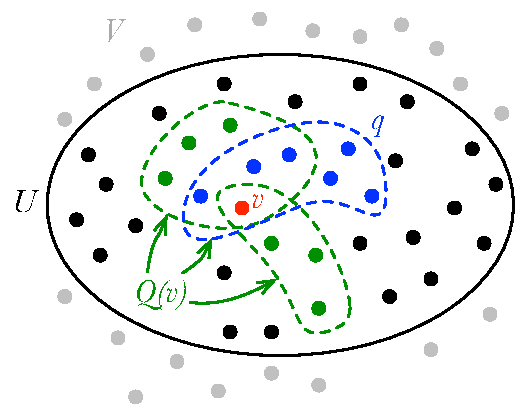
\includegraphics[width=8 cm]{Figures/vqQUV}
\caption{\bf \small The five levels of a Stellar network or FBAS}
\label{fig:vqQUV}
\end{figure}

Using the usual notation $2^X$ for the power set\footnote{The power set of a set $X$ is the set of all possible subsets of $X$ \cite{Cameron2008}. For a set of $N$ elements, its power set turns out to have $2^N$ elements, hence the notation.} of the set $X$, $2^V$ is the power set of $V$, i.e.\ the set of all possible quorum slices. At the next level, $2^{2^V}$ is the power set of quorum slices, i.e. the set of all possible \emph{sets} of quorum slices. Figure \ref{fig:SliceAndQ} shows a visualization of the elements of these kinds of power sets.

\begin{figure}[h]
\centering
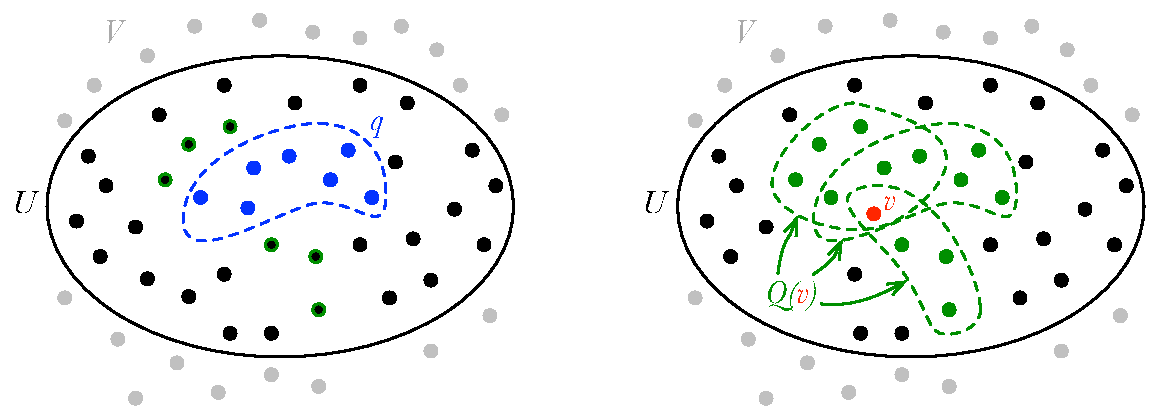
\includegraphics[width=15 cm]{Figures/SliceAndQ}
\caption{\bf \small LEFT: a) $q$ is an element of $2^V$. RIGHT: b) $Q(v)$ is an element of $2^{2^V}$.}
\label{fig:SliceAndQ}
\end{figure}

The function $Q$ assigns to each node $v \in V$ a set of slices $\{ q_1, q_2, \cdots, q_k \}$. Here the curly brackets denote set and $k$ is the number of slices for a given node $v$. Formally,
\begin{align}
Q\colon V \rightarrow 2^{2^V} \setminus \emptyset,
\end{align}
where $\setminus \emptyset$ means that the empty set is not in the range of this function ($Q(v)$ can never be empty).\footnote{It is not immediately clear whether this is a consequence of how this function operates or whether it is a requirement that we are adding arbitrarily to ensure that it does what we need. \textcolor{red}{TBD.}} In general,
\begin{align}
\forall v \in V, \forall q \in Q(v), \qquad v \in q,
\end{align}
which reads `For all nodes $v$ members of the set $V$ and for all slices $q$ members of the set $Q(v)$, node $v$ is a member of some slice $q$'.
\begin{defin}
A Federated Byzantine Agreement System \emph{(\textbf{FBAS})} is a pair $(V, Q)$.
\end{defin}
\begin{defin}
A set of nodes $U \subseteq V$ in a FBAS $(V, Q)$ is a \emph{\textbf{quorum}} iff $U \ne \emptyset$ and $U$ contains a slice for each member:
\begin{align}
\forall v \in U, \exists q \in Q(v) \ | \  q \subseteq U.
\end{align}
\end{defin}
In English: for all $v$ members of a quorum $U$, there exists a slice, member of $Q(v)$, such that the slice is a subset of, or equal to, the quorum $U$. A quorum can also be described as a set of nodes sufficient to reach agreement.
\begin{defin}
A \emph{\textbf{quorum slice}} $q$ is a subset of a quorum $U$ sufficient to convince a particular node $v$ of agreement.
\end{defin}
Therefore, a quorum slice is usually smaller than a quorum, as shown in the figures above. The `convincing' is depicted graphically by an arrow that depicts dependence between nodes in a manner analogous to inheritance in UML class diagrams. As shown in Figure \ref{fig:convincing}a, $v_2$ can convince $v_1$ but not vice versa, i.e.\ $v_1$ depends on itself and on $v_2$ while $v_2$ depends only on itself. Figure \ref{fig:convincing}b, shows the corresponding slices. Note that in this simple case the quorum of this set of nodes $V = \{ v_1, v_2 \}$ equals the slice for $v_1$: $V = U = q(v_1) = \{ v_1, v_2 \}$, whereas the set of slices $Q(v_1)$ is written $Q(v_1) = \{ \{ v_1, v_2 \} \}$, where the outer curly brackets indicate the set of slices $Q(v_1)$ and the inner curly brackets indicate the slice $q_1 = q(v_1)$.

\begin{figure}[h]
\centering
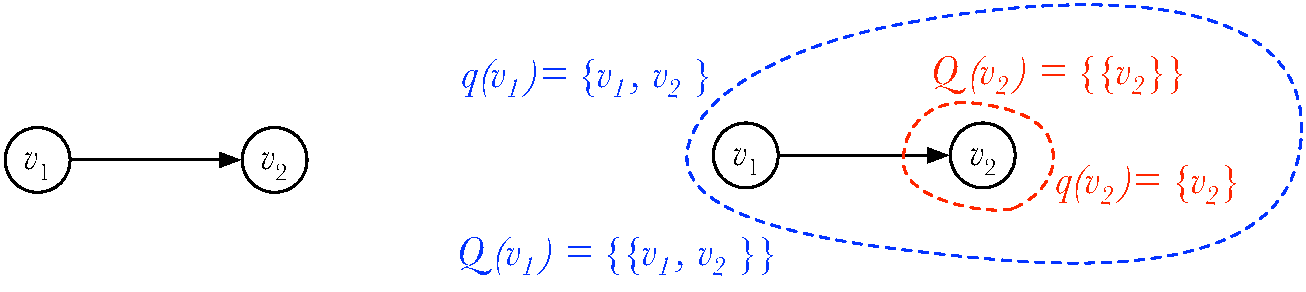
\includegraphics[width=15 cm]{Figures/convincing}
\caption{\bf \small LEFT: a) $v_2$ can convince $v_1$ but not vice versa. RIGHT: b) The slices of $v_1$ and of $v_2$.}
\label{fig:convincing}
\end{figure}

Figure \ref{fig:example1} shows a more complex interdependence between a set of 4 nodes. The arrows imply that $v_2$, $v_3$, and $v_4$ each has the same slice, e.g.\ $Q(v_2) = \{\{ v_2, v_3, v_4 \} \}$. In this example, although $\{\{ v_2, v_3, v_4 \} \}$ is a quorum, the smallest quorum involving $v_1$ must involve all four nodes.

\begin{figure}[h]
\centering
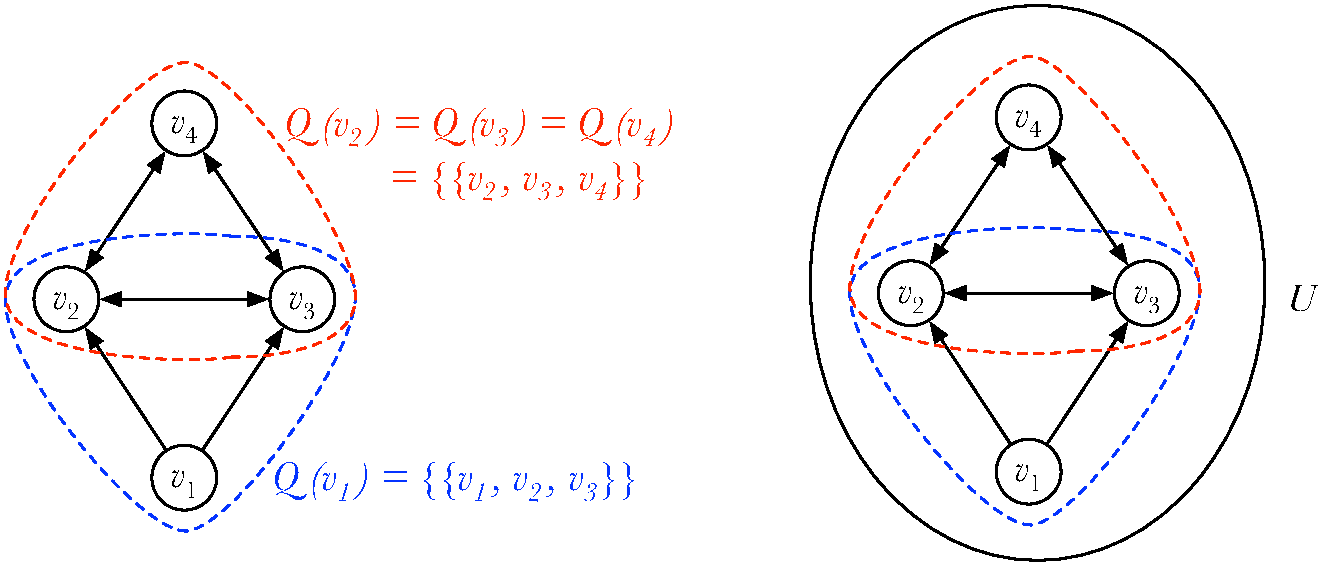
\includegraphics[width=15 cm]{Figures/example1}
\caption{\bf \small LEFT: a) The slices of this network. RIGHT: b) The smallest quorum involving $v_1$. (After \cite{Mazieres2016}).}
\label{fig:example1}
\end{figure}

In traditional, non-federated Byzantine systems all nodes have the same slices, i.e.
\begin{align}
\forall v_i, v_j \in V, \qquad Q(v_i) = Q(v_j). \qquad\qquad \text{[BAS]} 
\end{align}
Therefore, non-federated systems do not distinguish between slices and quorums. In our case, instead, in general we have that
\begin{align}
\forall v_i, v_j \in V, \qquad Q(v_i) \ne Q(v_j). \qquad\qquad \text{[FBAS]} 
\end{align}


















%\input{3-Functional_Requirements/funreq}
\chapter*{References}
\renewcommand{\section}[2]{}

\setlength{\parskip}{0.8\baselineskip}
\bibliographystyle{plainurl}
\small
\addcontentsline{toc}{chapter}{References}
\bibliography{Bib/BioComp_References}

%===================================================
%================== APPENDIX
%===================================================
%\begin{appendix}
%\section*{Appendix}
%\includepdf[pages={-}]{sections/4-CaSM/CaCycleAsm.pdf}
%\end{appendix}

\end{document}